\section{Analysis}
% \begin{figure}[!ht]    
    \centering
    % 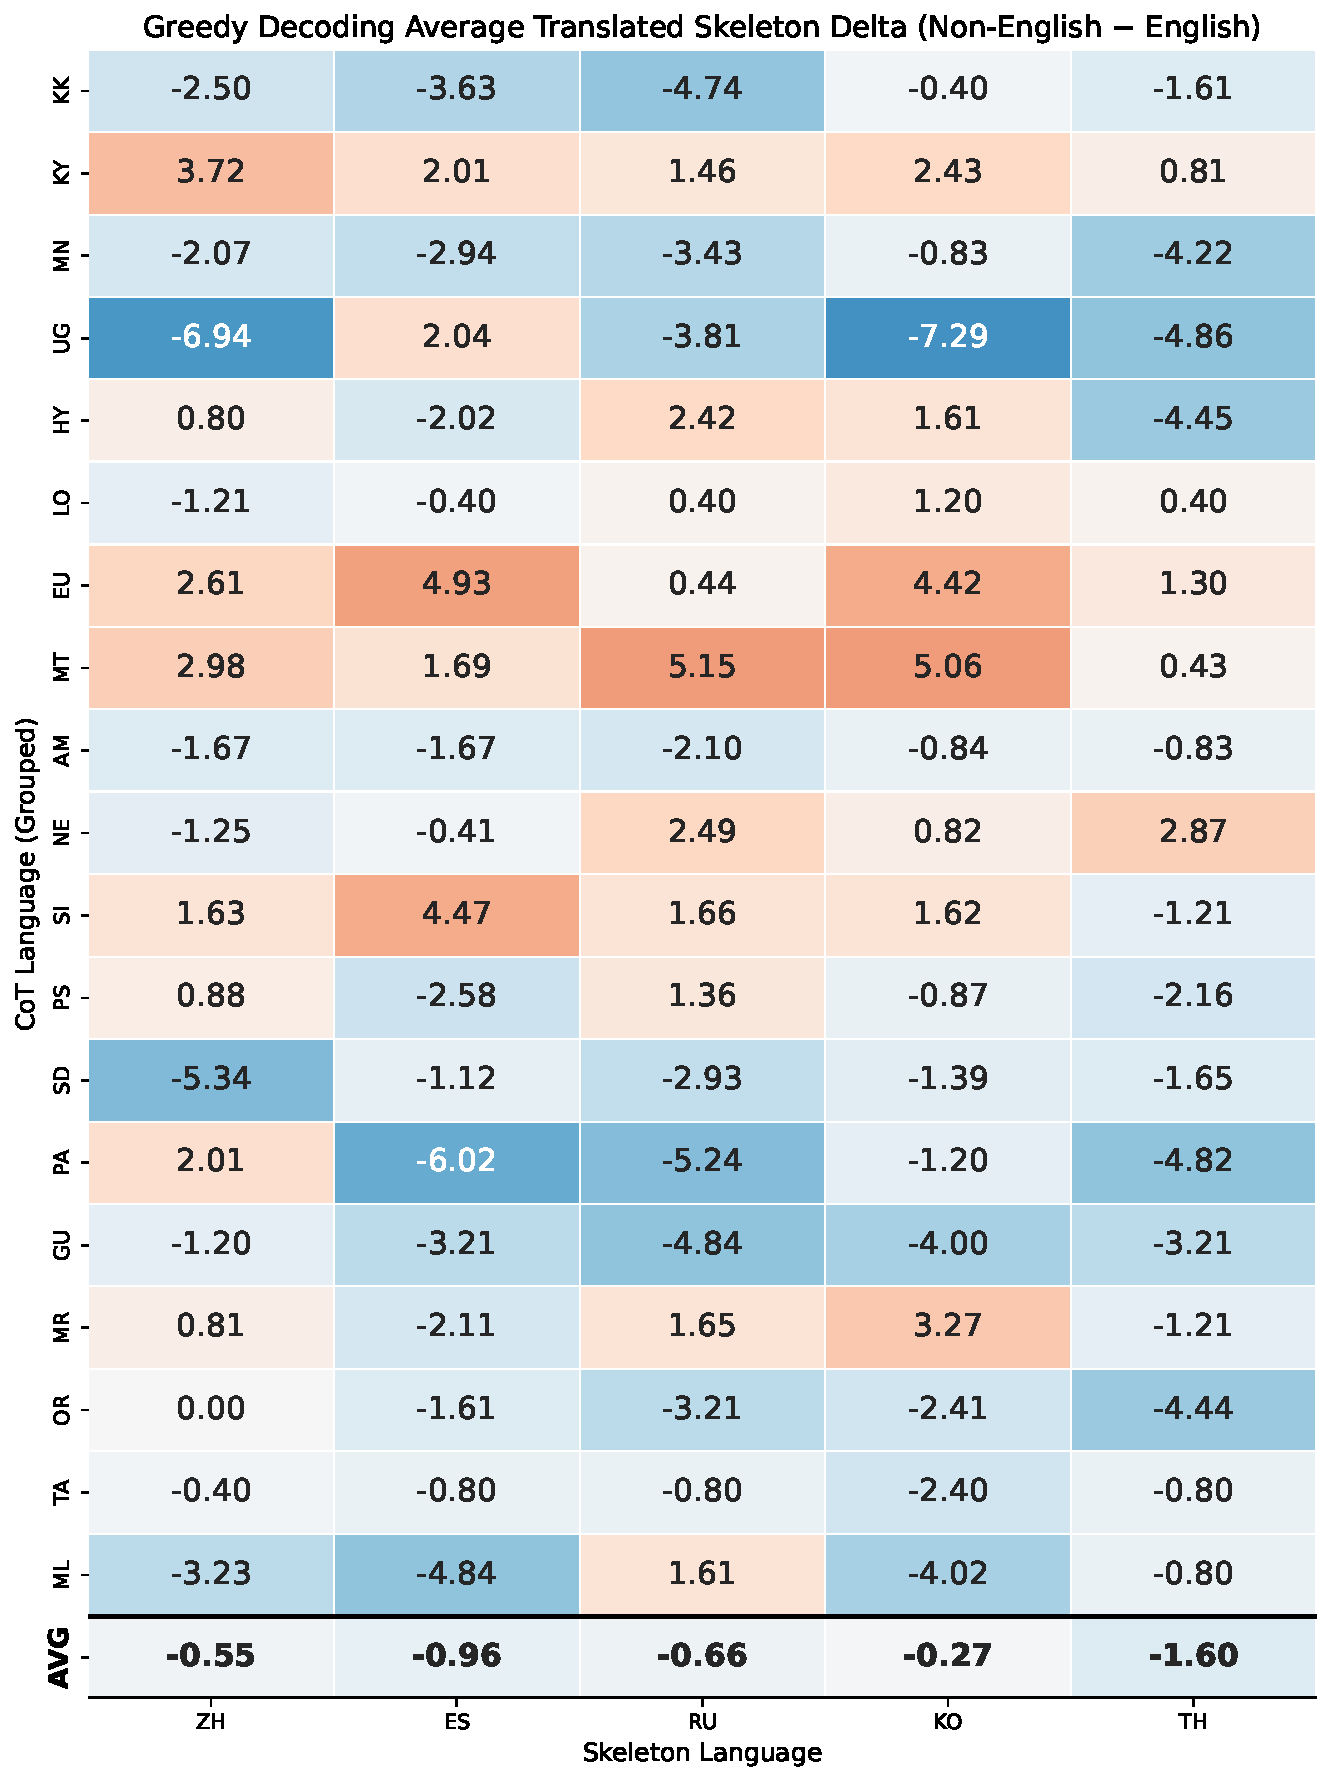
\includegraphics[width=\columnwidth]{Figures/Images/trans.pdf}
    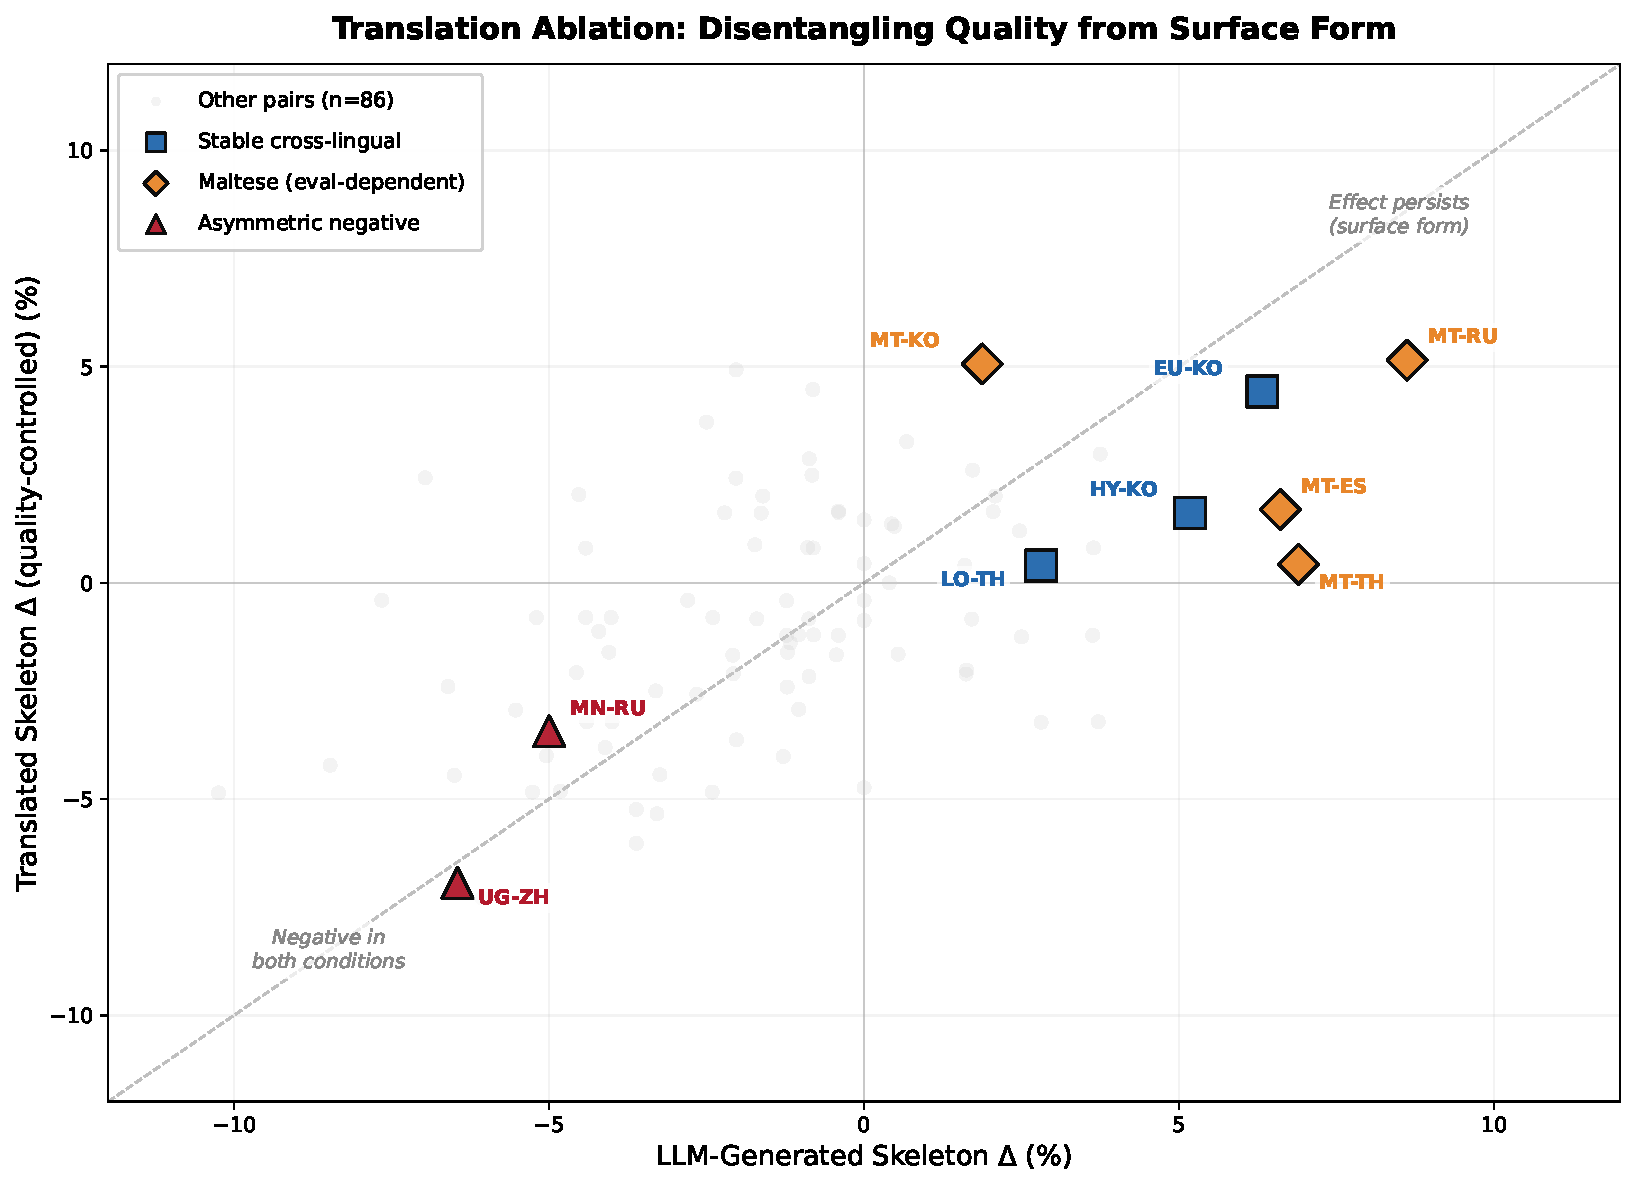
\includegraphics[width=\columnwidth]{Figures/Images/analysis_scatter_ablation.pdf}
    \caption{\small Translation ablation results. Each point is a (target, skeleton) pair, with $\Delta$ from LLM-generated skeletons on the x-axis and translated skeletons on the y-axis. Points near the diagonal indicate effects robust to skeleton quality.}
    \label{fig:translation_scatter}
    \vspace{-0.15in}
\end{figure}
In Section~\ref{sec:low-resource-nonen}, we observed that specific language pairs (e.g., Lao--Thai, Basque--Korean) can outperform reasoning approaches that utilize English skeletons. However, quantitative results alone are insufficient to pinpoint the precise causes of this performance improvement. Specifically, it remains unclear whether these gains stem from the superior generation quality of the skeletons themselves or from a synergistic effect arising from structural alignment with the target language.

In this section, to disentangle these factors, we conduct a criterion-based evaluation using an LLM-as-a-Judge. Specifically, we independently measure the Completeness, Specificity, and Coherence of the generated skeletons to analyze the correlation between skeleton quality and actual reasoning performance. Further details regarding the evaluation methodology are provided in Appendix~\ref{Appendix:skeleton_qualitative}.

We conducted a qualitative evaluation to determine whether the performance improvements observed in Section~\ref{sec:low-resource-nonen} for specific language pairs are attributable to the `Generation Quality' of the skeletons or to `Structural Alignment'.

\paragraph{Dominance of English Quality.}
As shown in Fig.~\ref{fig:lang_pair_heatmap}, regarding the intrinsic quality of skeletons across languages, English achieved the highest score~($7.57$), followed by Spanish~($7.35$), Chinese~($7.24$), and Russian~($7.13$). In contrast, Korean~($6.69$) and Thai~($5.65$) recorded relatively lower scores. This indicates that English, with its abundant pre-training data, serves as the most stable anchor in terms of skeleton generation capability, supporting the reason for the generally high performance of English observed in previous experiments (Section~\ref{sec:low-resource-nonen}).

% \paragraph{Quality-Performance Inversion.} However, an intriguing observation is the \textit{inversion} phenomenon between skeleton quality scores and actual reasoning performance. For Lao (lo), although the quality of Thai (th) skeletons (6.48) was 1.29 points lower than that of English (7.77), the actual reasoning performance using Thai skeletons was 2.81 points higher. Similarly, for Basque (eu), the Korean(ko) skeletons (6.18) lagged behind English (7.37) by 1.19 points in quality, yet resulted in a performance gain of 6.32 points. Conversely, this inversion was not observed in the absence of linguistic alignment. For Uyghur (ug), while the quality of Chinese skeletons (7.40) was comparable to English (7.54), performance dropped by 6.45 points. In the case of Mongolian (mn), although Russian skeletons (7.22) exhibited slightly higher quality than English (7.19), performance decreased by 5.53 points. These findings suggest that linguistic alignment can compensate for the deficit in skeleton quality.

\begin{figure}[!t]    
    \centering
    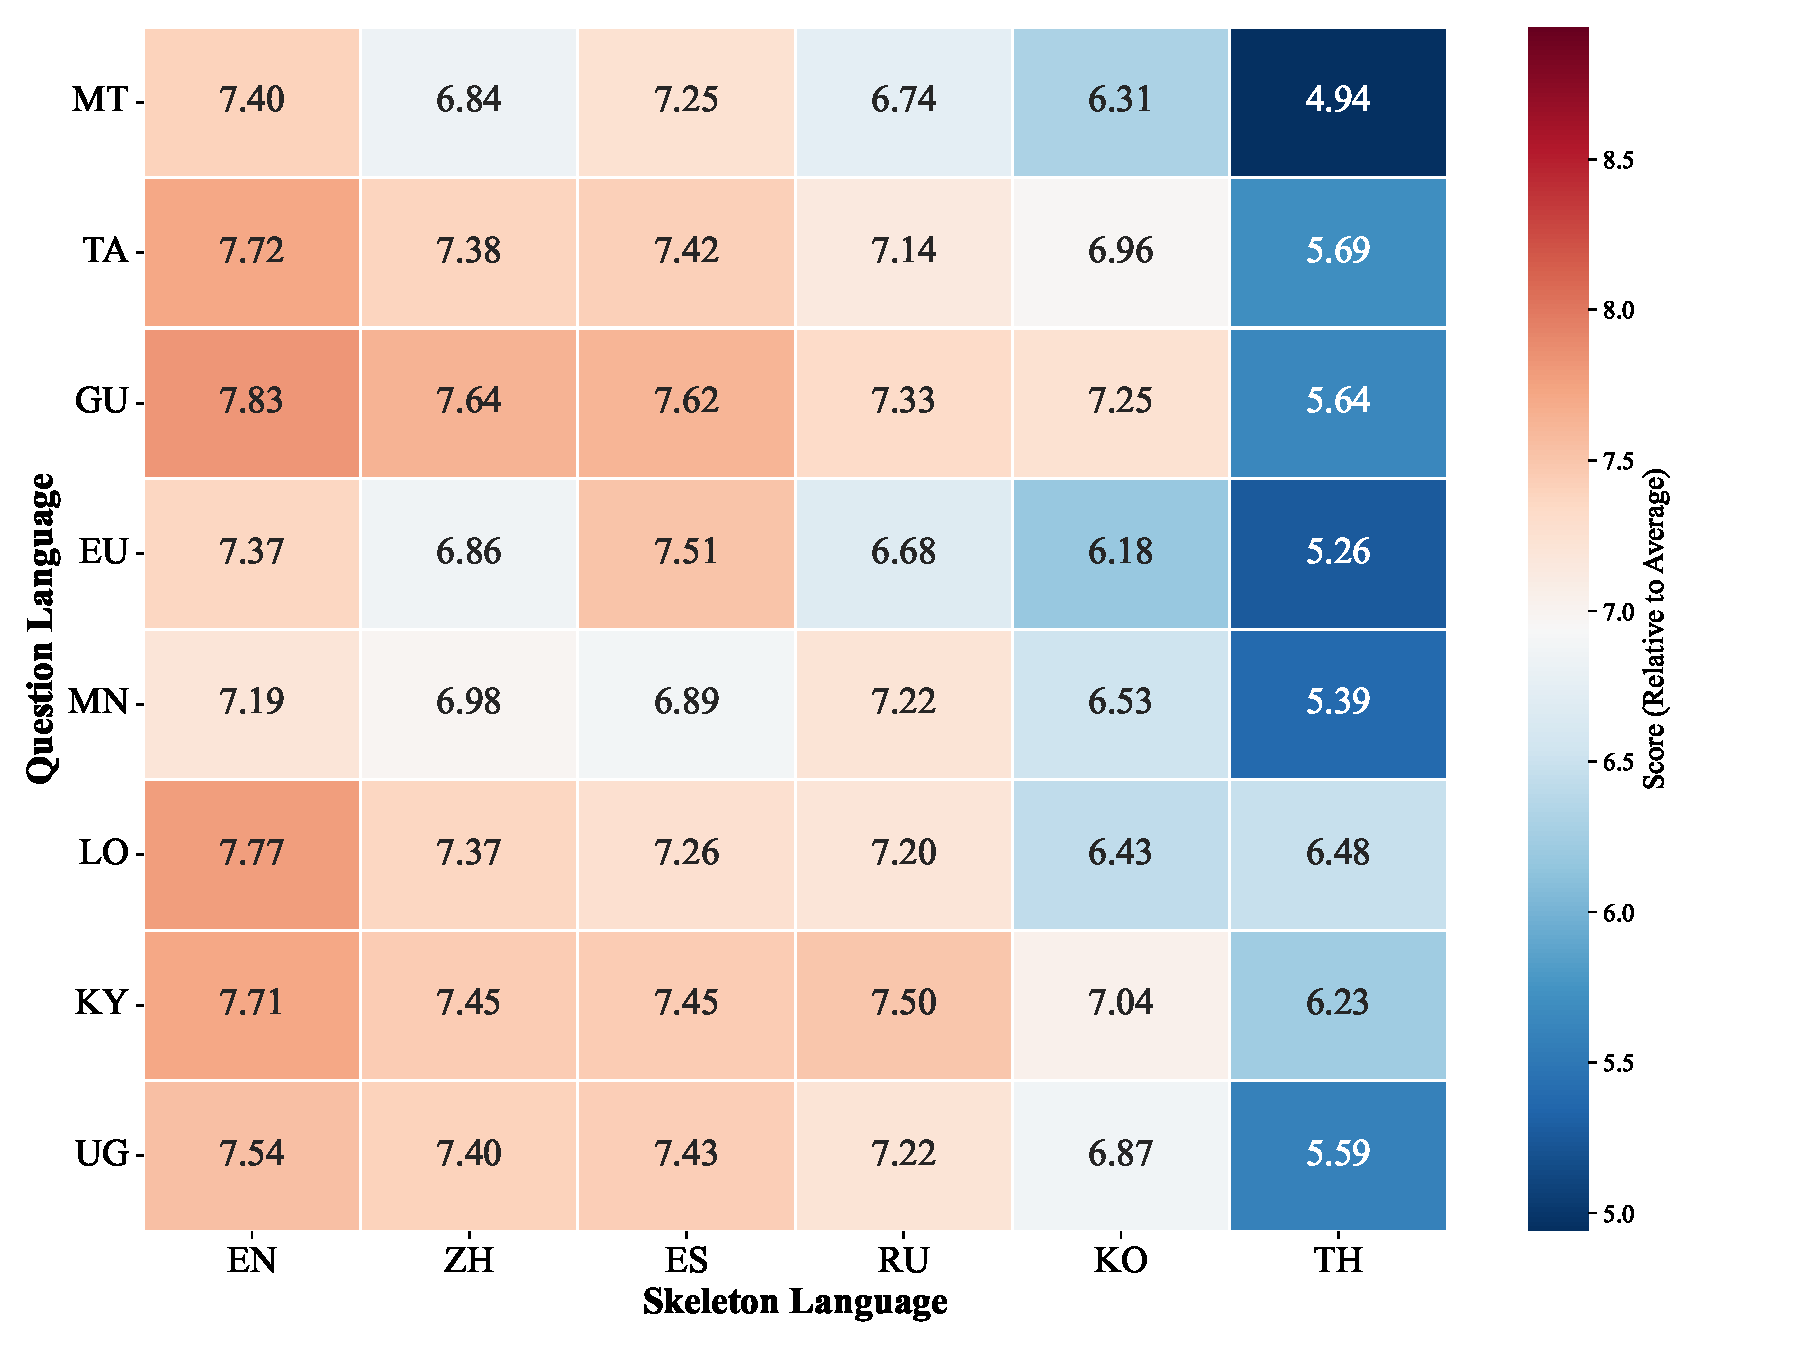
\includegraphics[width=\columnwidth]{Figures/Images/lang_pair_heatmap_styled.pdf}
    % 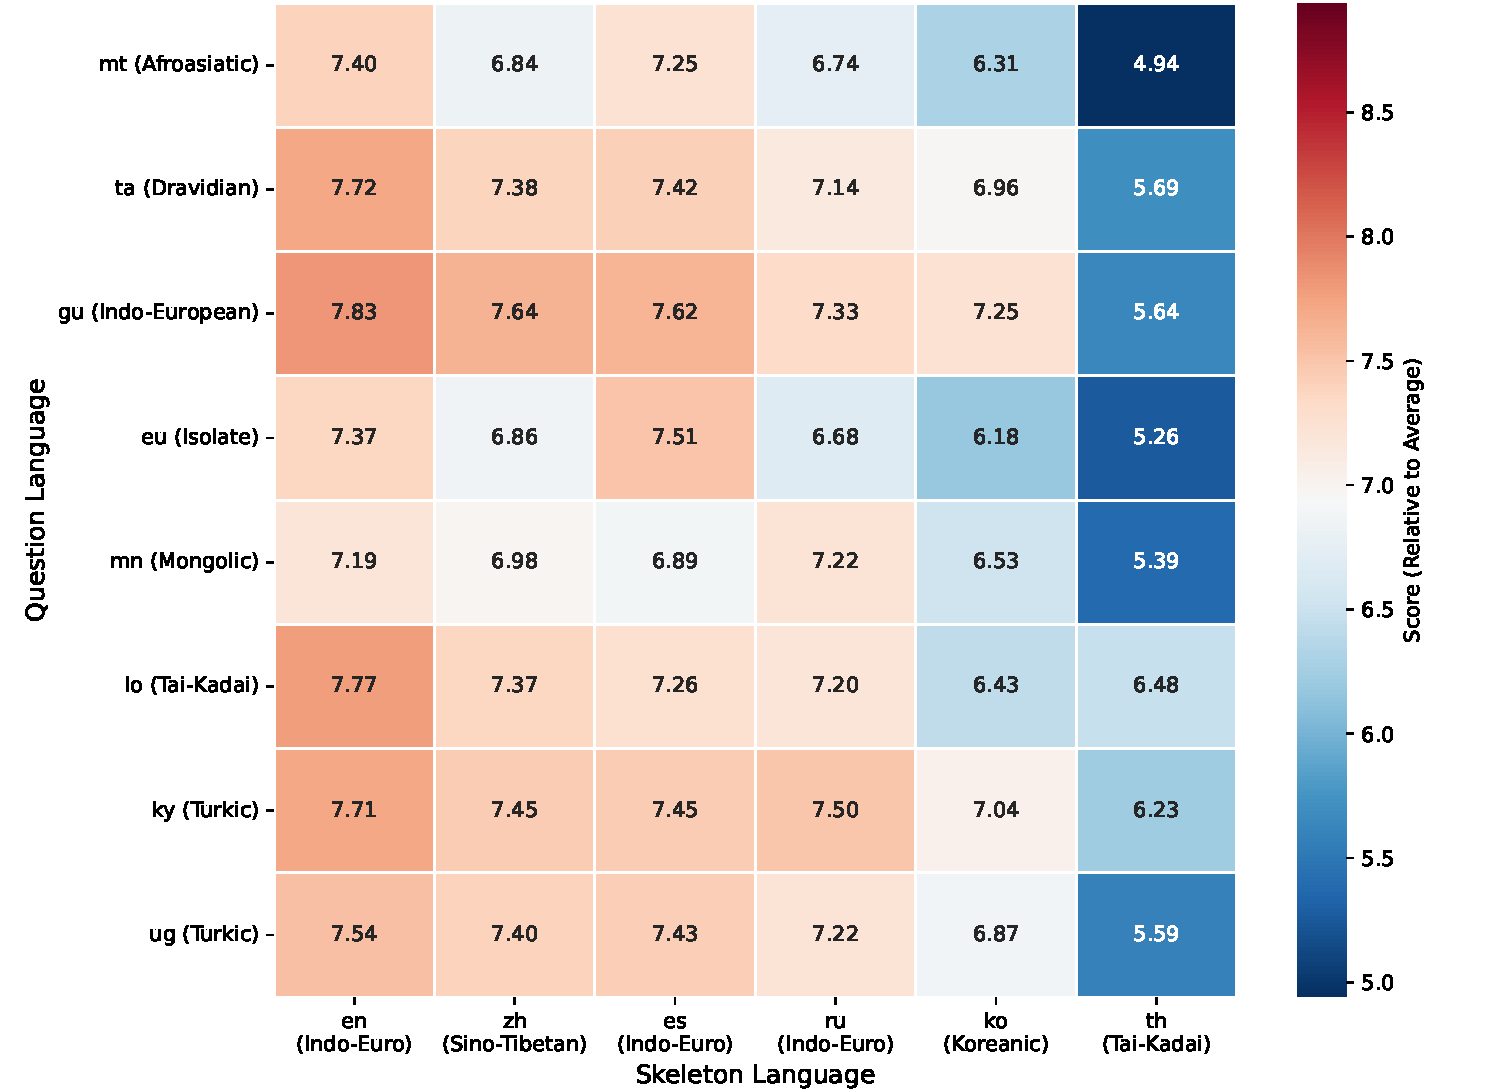
\includegraphics[width=\columnwidth]{Figures/Images/lang_pair_heatmap_cropped.pdf}
    \caption{\small Skeleton quality heatmap across language pairs. English skeletons yield highest quality (7.57), while Thai performs worst (5.65).}
    
\label{fig:lang_pair_heatmap}
    \vspace{-0.15in}
\end{figure}
\paragraph{Quality-Performance Inversion.} However, an intriguing observation is the \textit{inversion} phenomenon between skeleton quality scores and actual reasoning performance. For Lao~(lo), although the quality of Thai~(th) skeletons (6.48) was 1.29 points lower than that of English (7.77), reasoning performance using Thai skeletons was 2.81 points higher. Similarly, for Basque~(eu), the Korean~(ko) skeletons (6.18) lagged behind English (7.37) by 1.19 points in quality, yet resulted in a performance gain of 6.32 points. Conversely, this inversion was not observed in the absence of linguistic alignment. For Uyghur~(ug), while the quality of Chinese skeletons (7.40) was comparable to English (7.54), performance dropped by 6.45 points. In the case of Mongolian~(mn), although Russian skeletons (7.22) exhibited slightly higher quality than English (7.19), performance decreased by 5.53 points. These findings suggest that linguistic alignment can compensate for the deficit in skeleton quality.

\paragraph{Implication.} These findings on the Quality--Performance Mismatch strongly support the validity of \Lasef. If reasoning performance were solely proportional to the generation quality of the skeleton, English, with its high completeness, would consistently yield the optimal solution. However, our analysis demonstrates that a skeleton with structurally aligned attributes to the target language can outperform a higher-quality English skeleton, even if its intrinsic quality is somewhat lower. Furthermore, such ``hidden alignments'' are difficult to predict \textit{a priori} based on superficial quality metrics or simple linguistic classifications alone. Therefore, this suggests that the skeleton language should not be treated as a fixed component; rather, the combination of languages requires active exploration.